\section{Language Model}\label{sec:model}
In developing this DSL, we needed to have a clear understanding of the specific domain, and develop and appropriate domain model to guide our efforts.  Admittedly, there exist many possible models that can describe this area of policy and policy management, and the model that we chose to initially use is purposefully simple to help ease development and implementation efforts.  We did however provide arbitrary language-level extensibility to support future extension into more demanding policy implementation areas.

We developed this model to help us understand how policy-centric DSLs would be used, to visualize how the various elements are inter-related, and to clarify important areas upon which to focus effort.  Through this model, we were able to conceptualize the initial language structure and generate performance hierarchies, as well as to tailor expected DSL use.

\subsection{Expected Use}
In order to develop the appropriate DSL giving users the power and expressivity they need to easily express usage management concepts, we begin by developing a model describing how we expect it to be used, and by whom, identifying key functional and non-functional characteristics.  We use roles codified as actors to identify the primary user base, and link those roles to specific use cases we expect to be common in day to day DSL use.  We also identify common inputs and outputs from expected activities, and show how those input and output elements are related.  We finally specify the essential core structure of the DSL, as well as extension points and default implementations of those points.

In general day to day use, we expect that certain activities will be much more common that others.  For example, each \textit{policy} requires a \textit{context} in order to both be developed and to run.  That \textit{context} describes the actors using an artifact protected by a policy, the artifact itself, and the environment in which the artifact is both expected to be used (during policy design) and is being used (at evaluation).  That said, the expectation is that the number of policies is much greater than the number of contexts associated with those policies.

Likewise, we expect that the number of times a policy is evaluated is much greater than the number of times that policy is designed and created.  Policies should be read, evaluated, or combined with other policies frequently.  This gives us a magnitude ordering for these activities, where the number of supported contexts is much less than the number of created policies, which is in turn much less than the number of times that policy is evaluated or otherwise used.

This has specific implications on both the DSL syntax and performance profile.  For example, as it is much more common for policies to be evaluated than contexts to be created, our efforts and tuning the system and increasing performance are best focused on policy evaluation rather than contextual activities.  In a similar vein, the language itself should be as simple to comprehend as possible for policies at the expense of contextual elements if necessary.

\begin{figure}[!t]
\centering
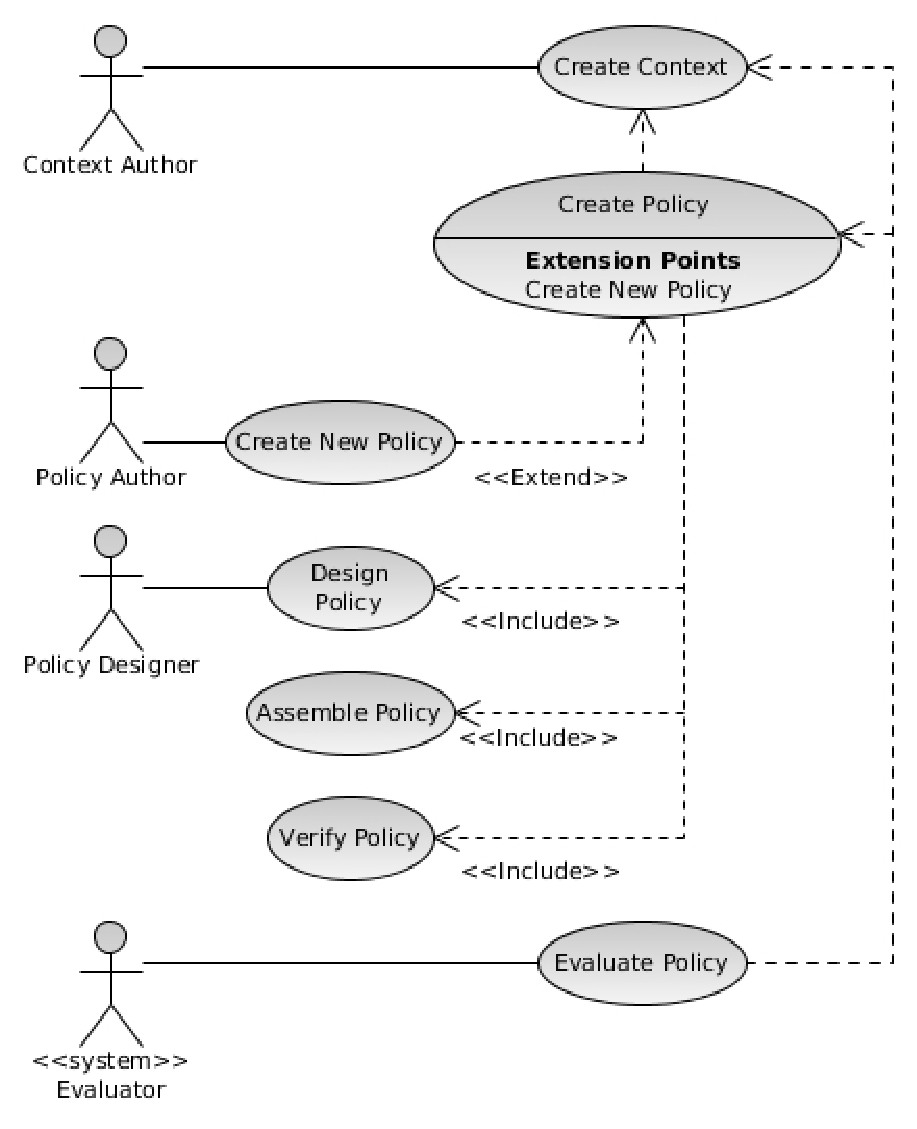
\includegraphics[width=3in]{use-cases}
\caption{General DSL Use Cases}
\label{fig:model:use-cases}
\end{figure}

Figure \ref{fig:model:use-cases} shows the primary system actors we have identified as well as the use cases with which they will be involved.  Actors include:
\begin{itemize}
\item \textit{Context Author}.  The context author is responsible for defining the context in which a policy will be applied to a given resource.  The context itself defines the environment in which the policy executes, the resource to which the policy is applied, and the subject that attempts to use the resource.
\item \textit{Policy Author}.  The policy author creates a policy to control the use of a subject defined in the policy context.
\item \textit{Combinator}. A system element, generally.  A combinator in this context combines two or more policies into a single composite policy.
\item \textit{Content Owner}.  The owner of a protected resource.
\item \textit{Evaluator}. Another system element, an evaluator evaluates a given policy with a specific context.
\end{itemize}

When a context author creates a context, that author compiles the elements of that context for use both at policy creation and policy execution.  When the policy is initially created, the resource is the only defined element.  Generally both the subject, representing the eventual user, and the environment, containing information describing the evaluation environment, are only defined at the classifier level.  That is to say, they both are defined, but individual properties have yet to be assigned.

Creating a policy is an activity undertaken by either a policy author or a combinator.  This step requires a \textit{declared} (but not \textit{defined}) context.  This is also undertaken in tandem with some kind of policy specification that describes roughly what the policy should manage and how it should be managed.  In the ontology we have defined, this is the step at which the author defines the various constraints, activities, restricted activities, and obligations.  Creating a new policy is precisely what it describes - creating a brand new policy applied to a context.  Creating a composite policy, on the other hand, involves creating a new derivative policy from two or more previously existing policies.

The included cases define policy, assemble policy, and verify policy are common development steps through which the policy is essentially designed, developed, and then tested against a context.

Once a policy has been created, the content owner can then associate that policy with a resource, essentially instantiating the resource in the associated context.

Finally, a policy is evaluated by an evaluator, a system actor, after creation and association with a resource.  At this point, the context has a fully instantiated context, with defined resource, subject, and environmental elements.

Now we have a general understanding of the expected use of a given policy, and have defined the expected roles.  With this in place, we begin to look at the elements the DSL should have to allow it to express the use cases we expect we need to support as the next step in refining our understanding of what this DSL should look like.

\subsection{Domain Ontology}
Our domain ontology will be the foundation of our DSL.  It will allow us to begin to understand the various language elements and how they are related, leading us to an eventual syntax to represent these classifiers and relationships.  Not understanding this structure well, or developing a structure that does not support our defined use cases will lead us to develop a DSL that inadequately supports our expected use.

Based on our use cases, we know the ontology contains a \textit{context}, some kind of policy-specific sub-ontology, and a logic engine that can act over that sub-ontology.  Based on our current understanding of our needs, the sub-ontology contains \textit{obligations} and \textit{constraints} applied to \textit{activities}.  We use simple propositional logic to reason over the policy elements.

This understanding leads us to the Ontology view in Figure \ref{fig:model:ontology}.  Of special note, the specific policy sub-ontology is represented as a realization of a more general \textit{policy ontology} type.  Likewise, the logic used to reason over the policy elements is propositional logic.  Both of these can change within this model to allow for inclusion of more complex policy systems and powerful reasoning capabilities.



\begin{figure}[!t]
\centering
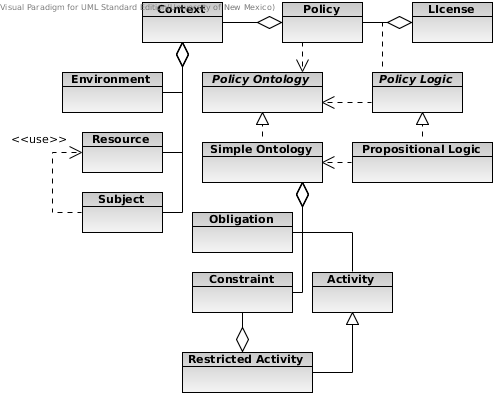
\includegraphics[width=3in]{ontology}
\caption{Basic Language Ontology}
\label{fig:model:ontology}
\end{figure}

\subsection{Envisioned Lifecycle}

\begin{figure}[!t]
\centering
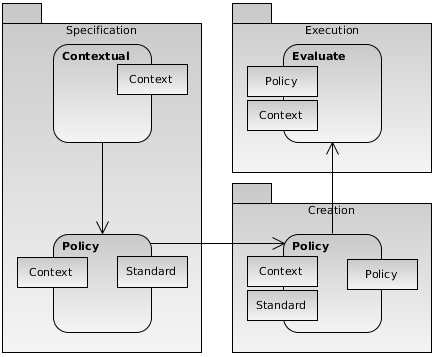
\includegraphics[width=3in]{lifecycle}
\caption{Policy Development Lifecycle}
\label{fig:model:lifecycle}
\end{figure}

\subsection{Language Components}

\begin{figure}[!t]
\centering
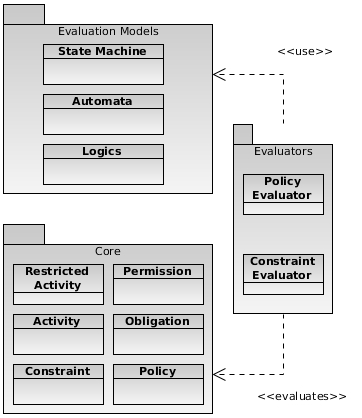
\includegraphics[width=3in]{language-components}
\caption{Language Elements}
\label{fig:model:language-components}
\end{figure}
